\chapter{Introduction}

Consider the lattice depicted in the leftmost diagram of Figure \ref{fig:simple_puzzle}. We refer to the elements of this lattice as \emph{cells}. Suppose we have the capacity to infect some cells (colored red) with a disease, and that this disease will, over a period of time, propagate through uninfected cells of the lattice. We define that uninfected cells become infected if they are exposed to at least two infected neighboring cells in the vertical and/or horizontal directions. We say that the initial infection is \emph{lethal} if the entire lattice ultimately becomes infected. Here is a puzzle:

\begin{question}
\label{que:simple_puzzle}
What is the fewest number of infected cells necessary to spawn a lethal infection?
\end{question}

\begin{figure}[]
\centering
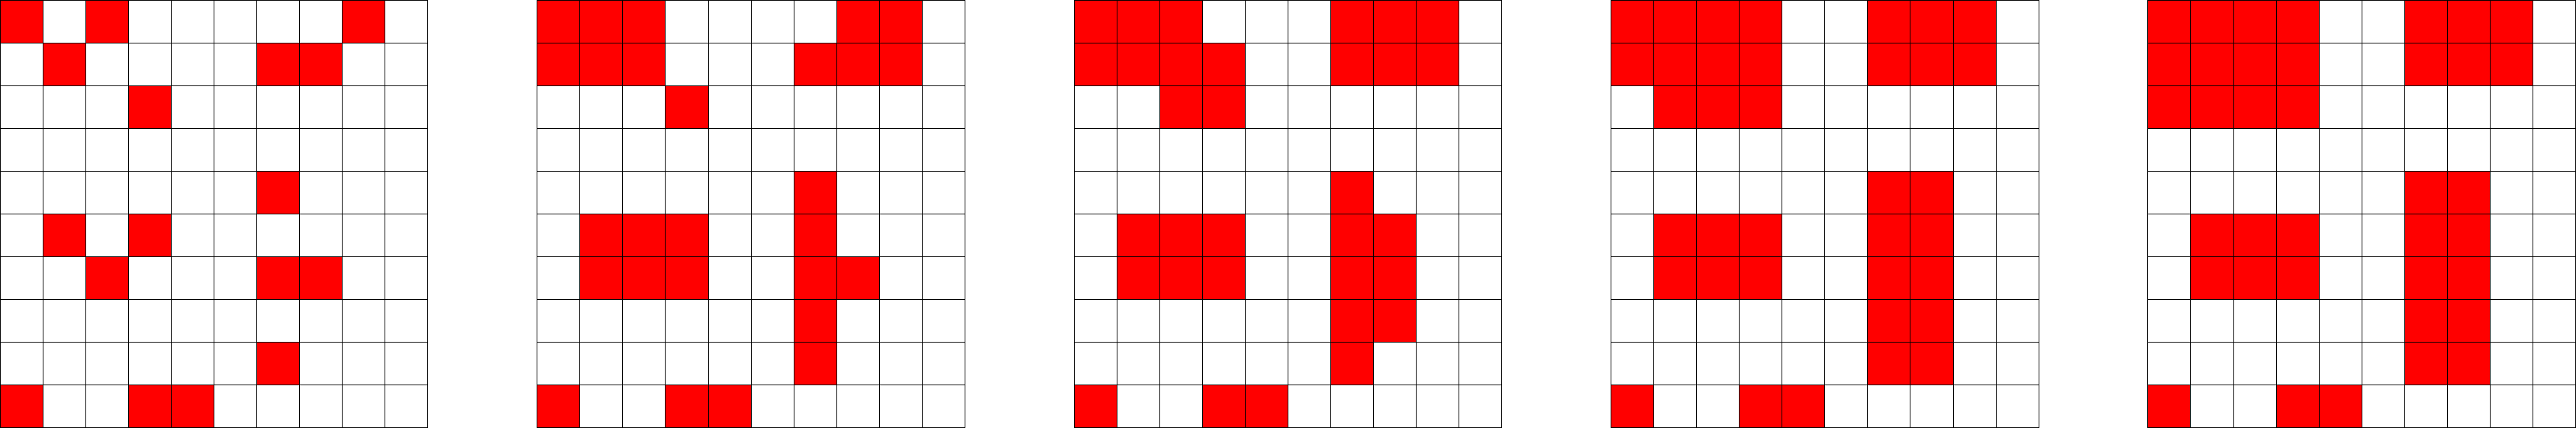
\includegraphics[width=\textwidth]{figures/1/simple_puzzle.pdf}
\caption{An arbitrary set of initially infected cells in the $10 \times 10$ lattice, and the stages of infection.}
\label{fig:simple_puzzle}
\end{figure} 

Before we present the solution,
%(which is particularly elegant and satisfying, and the reader is encouraged to play around with this problem on their own and get a feel for the behavior), 
let us take a moment to examine properties of sets of infected cells and attempt to identify some attributes which may correspond to lethality. It should not take too long to observe that if an initial infection is in some way ``spread too thinly," then it will be unable to ``jump" between infected areas, leading to gaps in infection or \emph{immune regions}. For example, an infection cannot cross any two consecutive uninfected columns or rows. In particular, the final image of Figure \ref{fig:simple_puzzle} contains an infected region in the upper right that cannot expand further due to being surrounded by too many uninfected cells. The perimeter of the lattice is particularly difficult to reach, as vertices there have fewer neighbors from which they might be exposed. Heuristically, then, a lethal set should have the ability to effectively span the entire lattice, and should be particularly virulent along the perimeter. 

With this criteria in mind, we are able to make educated guesses regarding the specific structure of sets that are likely to be lethal. In particular, we would like to consider the two starting infections illustrated in Figure \ref{fig:two_infections}. Notice that while Figure \ref{fig:two_infections} (\subref{fig:two_infections_b}) has far fewer perimeter infections, both (\subref{fig:two_infections_a}) and (\subref{fig:two_infections_b}) manage to form ``continuous bands" of infected cells that appear to span the entire lattice from the bottom left to top right after one step. Indeed, this fits with our notion of immune regions (or lack thereof), and we see that both infections propagate outwards from these bands until all cells become infected. However, we caution that no specific paradigm for the infection process should be taken as gospel; while heuristics are valuable, it is often easy to find lethal sets that violate them.

\begin{figure}[]
\centering
\begin{subfigure}{0.45\textwidth}
	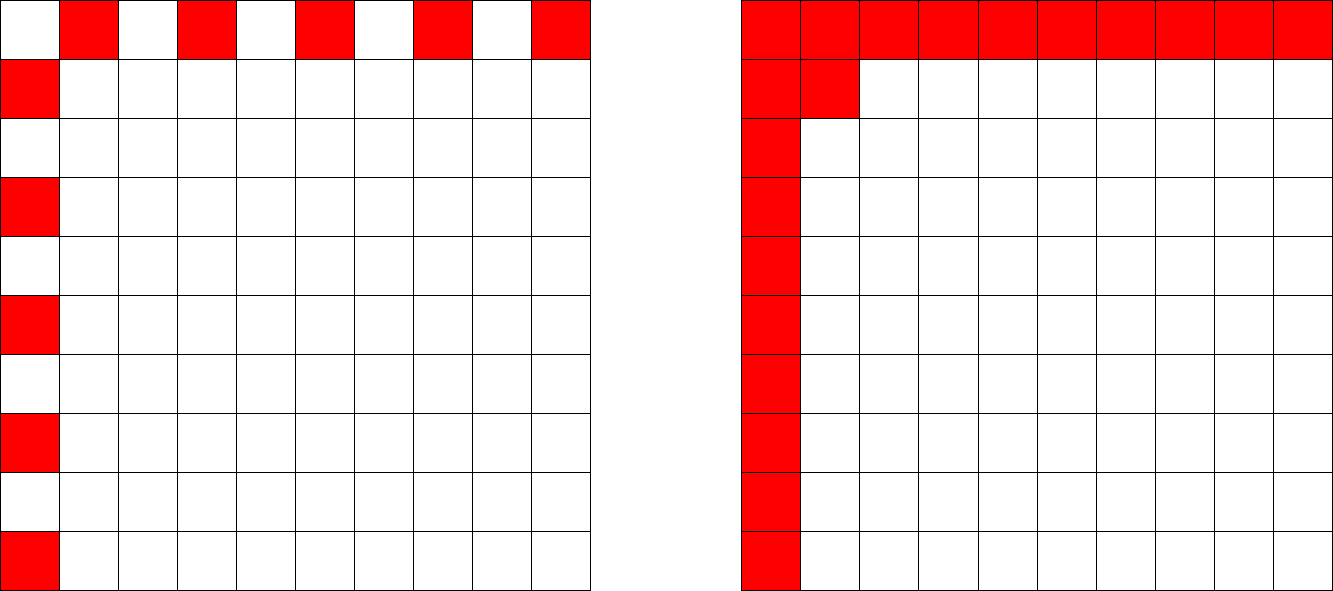
\includegraphics[width=\textwidth]{figures/1/two_infections_a.pdf}
	\caption{Perimeter construction.}
	\label{fig:two_infections_a}
\end{subfigure} \hfill%
\begin{subfigure}{0.45\textwidth}
	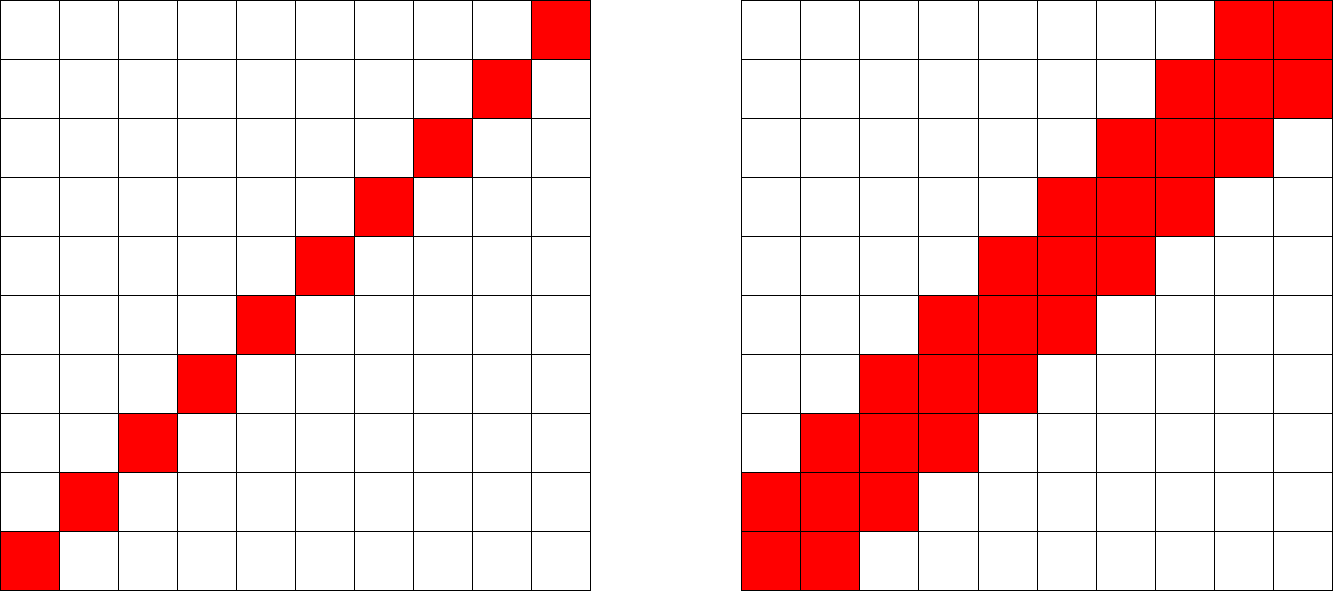
\includegraphics[width=\textwidth]{figures/1/two_infections_b.pdf}
	\caption{Diagonal construction.}
	\label{fig:two_infections_b}
\end{subfigure}
\caption{Two lethal sets and their resulting infections after one time-step.}
\label{fig:two_infections}
\end{figure} 

It is clear from Figure \ref{fig:two_infections} that we may obtain lethal sets on the $n \times n$ lattice of size $n$ by simply infecting the diagonal. What is less obvious is whether it is possible to improve upon this result. Perhaps a most natural first attempt at improvement is to remove an infection from one of the cells along the diagonal. However, this seems to form an immune region containing the removed cell. After some experimentation, one begins to believe it impossible to simultaneously satisfy the heuristic that a starting infection must span the lattice, while also using fewer than $n$ initial infections. The question therefore becomes: how do we prove it?

\subsection{An early result} \label{section:early_result}

We shall consider the cumulative perimeter of infected cells. 
%Let $G$ be an $n \times n$ grid graph, with vertex set $V = [n]^2$ and edges between adjacent vertices in the four cardinal directions. Consider $G$ to be embedded within the larger grid graph $G'$, where $V(G') = \{[n] \cup \{0, n+1\}\}$, and not 
For a given infectious set $A$, let $P(A)$ be the total perimeter of the infected cells of $A$. More precisely, we define $P(A)$ to be the number of sides of infected cells that \emph{do not} border other infected cells. Let $A_0$ be an initial infection, and observe that $P(A_0) \leq 4 |A_0|$. (This bound is only tight if no two infected cells are adjacent. Otherwise, the edge between such cells lies within the infected region, and cannot contribute to the infection's perimeter.) Observe that for any uninfected cell to become infected, it must abut at least two infected cells. Upon infection, the edges adjacent to these cells no longer lie on the infection's perimeter; additionally, the remaining edges of this newly infected cell contribute at most $2$ to this perimeter. All told, after infection, $P(A_1) \leq P(A_0)$, where $A_1$ is the set of cells infected after one time step.

If we suppose that $A_0$ is a lethal set, then at some point in time the entire grid will become infected. This infection will have perimeter $4n$. Since this perimeter cannot have increased, $A_0$ must have originally had a perimeter of at least $4n$. Since each cell in $A_0$ can contribute at most $4$ to this perimeter, it must be the case that $|A_0| \geq n$. Our diagonal construction shows that an optimal set $A_0$ satisfies $|A_0| \leq n$, and so we are able to conclude that $n$ is indeed best possible.

This proof is an instance of the famous \emph{perimeter argument}, which has belonged to bootstrap percolation folklore since at least the work of Pete \cite{pete:1997}. It also appears in the wonderful book \emph{The Art of Mathematics: Coffee Time in Memphis} by B\'ela Bollob\'as as Problem 34, along with similar questions in Problems 35, 65 and 66 \cite{bollobas2006coffee}. In the following section, we present additional well-known generalizations of this problem to higher dimensional rectangular grids.

\section{Bootstrap Percolation}

%Before presenting a proof, let us take a moment to formally define the process described above and develop some useful notation. 
The study of such cellular infection spread in grids (and, more generally, in graphs) is known in the literature as \emph{bootstrap percolation}, and was introduced in the 1970s by Chalupa, Leath and Reich as a simplified model for the behavior of ferromagnetic fields \cite{chalupa:1979}. In their original 1979 paper, the authors research the stable structure of probabilistically selected initial infections. While this differs from the problem posed in Question \ref{que:simple_puzzle}, the rules for the spread of infection and its broad behavior remain the same. It is worth noting that a large portion of contemporary research on bootstrap problems is focused on questions of probabilistic nature; while these problems are certainly interesting and of merit, they do not fall within the scope of this thesis. Rather, we shall focus on those problems where we have specific control over the structure of the initial infections; in particular, we aim to determine the smallest lethal set on the Cartesian product of paths and cycles. 

Let us now define the problem in concrete terms. Let $G$ be a graph, let $r \geq 0$ and let $A_0 \subseteq V(G)$ be a set of initially infected vertices. Iteratively, infect those vertices of $G$ with at least $r$ infected neighbors. For all $t > 0$, let $A_t$ be the set of infected vertices at time step $t$. We then have
$$A_t = A_{t-1} \cup \{v \in V(G) : |N_G(v) \cap A_{t-1}| \geq r\},$$
where $N_G(v)$ is the set of vertices adjacent to $v$ in $G$. We define the \emph{closure} of $A_0$ under $r$-neighbor bootstrap percolation to be $[A_0] = \bigcup_{t=0}^{\infty} A_t$. We say that $A_0$ \emph{percolates} or is \emph{lethal} if $[A_0] = V(G)$. We define the size of the smallest lethal set in a graph $G$ under $r$-neighbor bootstrap percolation by the quantity $m(G,r)$. We note that under these rules, it is not possible for vertices to become uninfected.

While it is possible to study bootstrap percolation on any graph $G$, much of the contemporary research focuses on multidimensional grids \cite{pete:1997,przykucki:2019,balogh:2006,benevides:2021,benevides2015maximum,benevides2013slowly,pete1997make,balogh2012sharp,balogh2009bootstrap,balogh2009majority,balogh2010bootstrap}. We therefore introduce the following notation. For all $n \in \mathbb{N}$, let $[n] = \{1, 2, \dots, n\}$. We denote by $\prod_{i=1}^d [a_i]$ the grid graph with vertex set $\prod_{i=1}^d [a_i]$ and edges between vertices that differ by 1 in exactly one coordinate. Note that $\prod_{i=1}^d [a_i] = P_{a_1} \square \cdots \square P_{a_d}$, where $\square$ denotes the Cartesian product of graphs, and $P_k$ denotes a path on $k$ vertices. Furthermore, define:
$$m(a_1, \dots, a_d, r) = m\left(\prod_i^d [a_i], r\right).$$

There are a number of natural generalizations of the problem posed in Question \ref{que:simple_puzzle}. In this thesis, we discuss those obtained by varying the structure of $G$ and the value of $r$. Below, we outline some of the existing results for graphs that are the Cartesian product of paths and cycles, and $r \in \{0, 1, 2, 3\}$. Some of these results are summarized in Table \ref{tab:known_bounds}.

\begin{table}[]
\centering
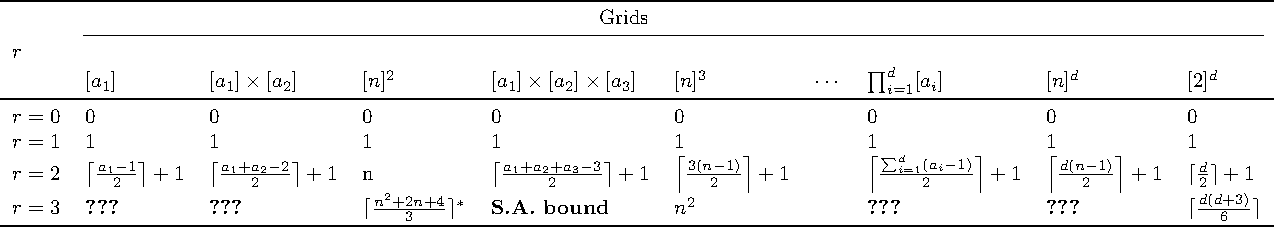
\includegraphics[width=\textwidth,origin=c]{tables/1/known_bounds.pdf}
\caption{A summary of known bootstrap percolation results for grids, $r \in \{0,1,2,3\}$.}
\label{tab:known_bounds}
\end{table} 

\subsection{Results on grids and tori}
\label{sec:result_summary}

In this section, we highlight existing extremal bootstrap percolation results on grids and tori. Some of the following bounds are not known to be tight and require supplemental constructions, which are often difficult to obtain. We further sub-divide this discussion into results on the grid (of which there are many), and results on the torus (of which there are few).

\subsubsection{Grids}

From the puzzle posed in Question \ref{que:simple_puzzle}, we readily obtain variant problems by altering three parameters: the size and shape of the grid $G$, the grid's dimension $d$, and the threshold number of neighbors $r$. We examine each of these problems in turn.

In the prior discussion of the perimeter argument, we showed that, for square grids, it holds that $m([n]^2, 2) \geq n$, and verified this to be tight with a diagonal construction. The following result (attributed to Pete \cite{pete1997make}) generalizes this result to all rectangular grids $[a_1] \times [a_2]$. A proof is included for completeness. 

\begin{thm}
\label{thm:perimeter_rects}
For $a_1, a_2 \geq 1$,
$$m(a_1,a_2,2) = \ceil*{\frac{a_1+a_2}{2}}.$$
\end{thm}

\begin{proof}
We obtain a lower bound on $m(a_1,a_2,2)$ by applying the perimeter argument. Note that the perimeter of the $a_1 \times a_2$ grid is $2(a_1+a_2)$, and so the $m(a_1,a_2,2) \geq \ceil*{\frac{a_1+a_2}{2}}$. (We take the ceiling because the size of infected sets must be integral. See Figure \ref{fig:sa_construction_2d}.) For the upper bound, we proceed by induction on $a_1+a_2$. For $a_1+a_2 \leq 4$, the lethal sets in Figure \ref{fig:base_cases} match the lower bounds given by the perimeter argument (1, 2, 2, and 2, respectively). For $a_1+a_2 > 4$, suppose without loss of generality that $a_1 \leq a_2$, and so $a_2 \geq 3$. By hypothesis, $[a_1] \times [a_2-2]$ admits a lethal set $A_0$ at the perimeter bound. We show that $A_0$, plus the addition of any infection in the final column of $[a_1] \times [a_2]$, is lethal and matches the perimeter bound. 

Observe that $A_0$ infects all vertices of $[a_1] \times [a_2]$, apart from the final two columns. The additional vertex in the final column is then sufficient to infect all remaining healthy vertices. Finally, by incrementing $a_2$ by two, the perimeter bound is incremented by exactly one. This completes the proof.
\end{proof}

\begin{figure}[]
\centering
\hspace*{\fill}
\begin{subfigure}{0.03\textwidth}
	
\includegraphics[width=\textwidth]{figures/1/1x1x1.pdf}
\end{subfigure} \hfill%
\begin{subfigure}{0.064\textwidth}
	
\includegraphics[width=\textwidth]{figures/1/1x2x1.pdf}
\end{subfigure} \hfill%
\begin{subfigure}{0.1\textwidth}
	
\includegraphics[width=\textwidth]{figures/1/1x3x1.pdf}
\end{subfigure} \hfill%
\begin{subfigure}{0.06\textwidth}
	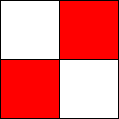
\includegraphics[width=\textwidth]{figures/1/2x2x1.pdf}
\end{subfigure}
\hspace*{\fill}
\caption{Tight constructions for lethal sets where $a_1+a_2 \leq 4$.}
\label{fig:base_cases}
\end{figure} 

Let us take a moment to examine the issue of integrality in the perimeter bound. When non-integrality occurs, either adjacent vertices are infected in the same generation, or a vertex is infected by more than $r$ neighbors. Note that in both cases, this decreases the perimeter of infection. One way to think about this is to consider each vertex as having ``infectious potential": vertices $v \in A_0$ can infect up to $d(v)$ healthy vertices, whereas vertices $v \in A_i$ for $i > 0$ can infect at most $d(v) - r$. An integral perimeter bound mandates that each vertex realize its potential, whereas a non-integral bound leaves a small margin for error. Figure \ref{fig:sa_construction_2d_a} illustrates the integral case, where each cell is infected by exactly two neighboring cells; this condition ensures that $P(A_i) = P([A_0])$ for all $i$. Conversely, in Figure \ref{fig:sa_construction_2d_b}, the cell demarcated with an ``X" experiences infection on three sides, thereby reducing its infectious potential. The existence of such a cell is guaranteed by the fact the perimeter bound in this case is non-integral. 

\begin{figure}[]
\centering
\begin{subfigure}{0.4\textwidth}
	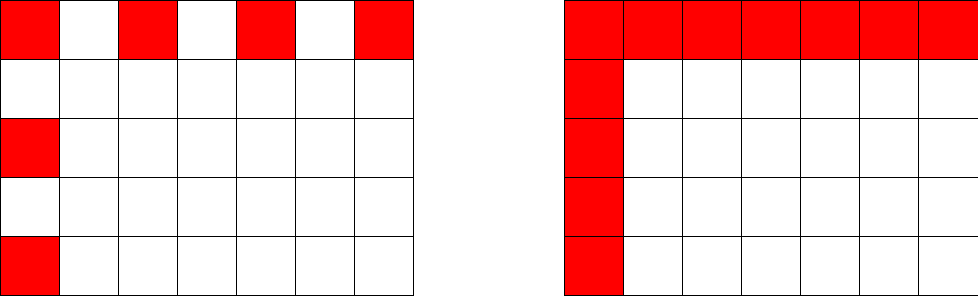
\includegraphics[width=\textwidth]{figures/1/5x7x1.pdf}
	\caption{$a+b \equiv 0 \pmod 2$}
	\label{fig:sa_construction_2d_a}
\end{subfigure} \hfill%
\begin{subfigure}{0.45\textwidth}
	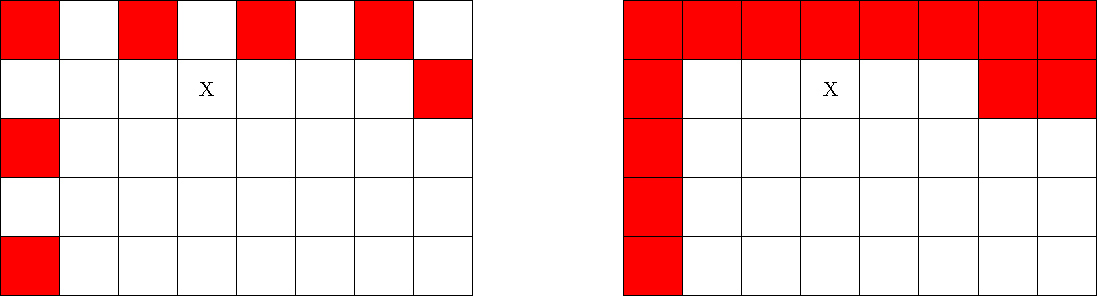
\includegraphics[width=\textwidth]{figures/1/5x8x1.pdf}
	\caption{$a+b \equiv 1 \pmod 2$}
	\label{fig:sa_construction_2d_b}
\end{subfigure}
\caption{Tight constructions for lethal sets on the $[a] \times [b]$ grid.}
\label{fig:sa_construction_2d}
\end{figure} 

We can further generalize in the case where $r=2$. In 2006, Balogh and Bollob\'as \cite{balogh:2006} proved the following general form of Theorem \ref{thm:perimeter_rects} for all $d$-dimensional grids $(a_1, \dots, a_d)$, $a_i \geq 1$:

\begin{thm}[Balogh and Bollob\'as]
\label{thm:complete_r_2}
For $d \geq 1$ and $a_1, \dots, a_d \geq 1$, 
$$m(a_1, \dots, a_d, 2) = \ceil*{\frac{\sum_{i=1}^d (a_i-1)}{2}}+1.$$
\end{thm}

Theorem \ref{thm:complete_r_2} completes the picture for infections with a threshold of two on grids. We now ask whether similar results exist for larger $r$. Unfortunately, while generalizing to $d$-dimensional grids yields nice results for $r=2$, attempts to obtain a holistic understanding of $m(a_1, \dots, a_d, r)$ for arbitrary $r$ have been largely fruitless. Even the case of $r=3$ remains stubbornly inaccessible for nearly all large $d$. However, certain breakthroughs have been made for $d=2$, $d=3$, and $G=[2]^d$.

We first consider 3-neighbor percolation on two-dimensional square grids. In 2021, Benevides, Bermond, Lesfari and Nisse proved that 
$$m(n,n,3) = \ceil*{\frac{n^2+2n+4}{3}}$$
for even $n$, and 
$$\ceil*{\frac{n^2+2n}{3}} \leq m(n,n,3) \leq \ceil*{\frac{n^2+2n}{3}} + 1$$
for odd $n$. Additionally, they showed that these bounds are tight in the following cases: if $n = 5 \pmod 6$, or $n = 2^k - 1$ for some $k \in \mathbb{N}$, then $m(n,n,3) = \ceil{\frac{n^2+2n}{3}}$; and if $n \in \{9,13\}$, then $m(n,n,3) = \ceil{\frac{n^2+2n}{3}} + 1$. Constructions that achieve this bound are illustrated in Chapter 5. We add to this picture with the following theorem, proven in Chapter 5, and corollary:

\begin{thm}
\label{thm:2d_rectangle}
Suppose that $a, b \geq 1$ such that
$$m(a,b,3) = \frac{2ab+a+b}{3}.$$
Then there exists $k \geq 1$ such that $a=b=2^k-1$.
\end{thm}

\begin{cor}
\label{cor:square_grids_thickness_1}
For all $n \geq 1$,
$$ m(n,n,3) =
\begin{cases} 
      \ceil*{\frac{n^2+2n+4}{3}} & n \equiv 0 \pmod 2; \\
      \frac{n^2+2n}{3} & n = 2^k-1, \; k \in \mathbb{N}; \\
      \frac{n^2+2n+1}{3} & n \equiv 5 \pmod 6; \\
      \frac{n^2+2n+3}{3} & \text{otherwise.}
   \end{cases}
$$
\end{cor}

\begin{proof}
The first three cases follow from Theorem 1 of \cite{benevides:2021} and the observation that if $n \equiv 5 \pmod 6$, then $\ceil{\frac{n^2+2n}{3}} = \frac{n^2+2n+1}{3}$. In the final case, $n$ is congruent to either 1 or 3 modulo 6. This implies that $n^2 + 2n$ is divisible by three. From Theorem 1 of \cite{benevides:2021}, we have that $m(n,n,3) \leq \frac{n^2+2n+3}{3}$. Furthermore, since $n$ is not of the form $2^k-1$, it follows from Theorem \ref{thm:2d_rectangle} that $m(n,n,3) > \frac{n^2+2n}{3}$. Therefore, $m(n,n,3) = \frac{n^2+2n+3}{3}$.
\end{proof}

This result resolves the question of the minimum lethal set for two dimensional square grids. For the more general case of rectangular grids, the problem remains unsolved. However, our experimentation suggests that nearly all grids $[a_1] \times [a_2]$ for $a_1,a_2 > 2$ fall within a constant factor of the bound given in Theorem \ref{thm:sa_bound}, below.
%However, we are able to achieve an upper bound of $m(a,b,3) \leq \ceil{\frac{ab+a+b+6}{3}}$ and a lower bound (described below) of $m(a,b,3) \geq \ceil{\frac{ab+a+b}{3}}$, for all $a,b > 1$. Further discussion of these results can be found in Chapter 6.

One significant and well-known result for $d$-neighbor percolation on $d$-dimensional grids is the following lower bound, taken as a $d$-dimensional analog of the perimeter bound. This result is referenced frequently throughout this document, and referred to interchangeably as the \emph{surface area} or \emph{SA bound}. We shall use the shorthand notation $SA(G)$ to refer to the surface area bound of a grid $G$. We prove the statement in full generality, while noting that we only make use of the case where $d=3$. We also note that, like the perimeter bound, the following proof belongs to bootstrap percolation folklore. While it appears to have been first published in 1997 by Balogh and Pete \cite{balogh1998random}, variations also appear in \cite{bollobas2006coffee,pete:1997,pete1997make}.

\begin{thm}
\label{thm:sa_bound}
For any $d \geq 1$ and $a_1, a_2, \dots, a_d \geq 1$, 
$$m(a_1,a_2, \dots, a_d,d) \geq \frac{\sum_{j=1}^d \prod_{i \neq j} a_i}{d}.$$
\end{thm}

\begin{proof}
We apply the same ``invariant" strategy presented in the perimeter argument. For simplicity, consider $\prod_{i=1}^d[a_i]$ to be embedded within the larger graph $\prod_{i=1}^d \{0, \dots, a_i + 1\}$. Note that in $\prod_{i=1}^d \{0, \dots, a_i + 1\}$, each vertex $v \in \prod_{i=1}^d[a_i]$ has degree $2d$. Let $A_0$ be a lethal set in $\prod_{i=1}^d[a_i]$ under the $d$-neighbor bootstrap process. For $t >0$, let $A_t$ be the set of infected vertices in $\prod_{i=1}^d[a_i]$ at generation $t$. Denote by $m_t$ the number of edges between vertices $u \in A_t$ and $v \in \prod_{i=1}^d \{0, \dots, a_i + 1\} \setminus A_t$. %We show that the sequence $m_0, m_1, m_2, \dots$ is monotonically decreasing. 
We show that $m_{t-1} \geq m_t$ for all $t> 0$. 

%Let $N = |A_t - A_{t-1}|$, and let $v_1, \dots, v_N$ be an arbitrary ordering on the vertices of $A_t \setminus A_{t-1}$. 
By definition, each vertex $v \in A_t \setminus A_{t-1}$ has at least $d$ neighbors in $A_{t-1}$. Therefore, since $d(v) = 2d$, $v$ has no more than $d$ neighbors outside of $A_t$. This implies that the number of edges from $A_{t-1} \cup \{v\}$ to $\prod_{i=1}^d \{0, \dots, a_i + 1\} \setminus A_{t-1} \cup \{v\}$ cannot exceed $m_{t-1}$. Furthermore, this holds for every vertex $v \in A_{t-1}$, and so $m_{t-1} \geq m_t$. 

Since $A_0$ is lethal, we have that 
$$2d|A_0| \geq m_0 \geq m_1 \geq \dots \geq 2 \sum_{j=1}^d \prod_{i \neq j} a_i,$$ 
where the final expression gives the total number of edges between the fully infected grid and the surrounding larger grid. Dividing through by $2d$ gives the result.
\end{proof}

We note that the prior argument is precisely the same as the so-called perimeter argument outlined in Section \ref{section:early_result}. Here, the quantity $m_t$ is a $d$-dimensional analogue of the perimeter of infection $P(A_t)$ at time-step $t$, and the lower bound
$$2\sum_{j=1}^d \prod_{i \neq j} a_i$$
is the $d$-dimensional ``perimeter" of the grid. Again, observe that equality can only be obtained when no vertices of $A_0$ are adjacent, and all vertices $v \in A_{t}$, for $t>0$, are infected by exactly $d$ neighbors. Any defect causes a reduction in ``perimeter" of two units, corresponding to a $1/d$ increase in the bound. 

We note that in the case where $a_1 = \dots = a_d = n$, the bound given in Theorem \ref{thm:sa_bound} simplifies to $m(n, \dots,n,d) \geq n^{d-1}$. Somewhat surprisingly, although it is not too difficult to find sets that meet this bound and appear to be lethal, verifying this claim is non-trivial. To the best of our knowledge, the first published proof of this fact appears in a 2019 paper by Przykucki and Shelton \cite{przykucki:2019}. 

\begin{thm}[Lower bound \cite{balogh1998random}. Upper bound \cite{przykucki:2019}]
\label{thm:hypercubes}
For all $n,d \geq 1$,
$$m(\underbrace{n,\dots,n}_d,d) = n^{d-1}.$$
\end{thm}

The primary aim of this thesis is to prove that the surface area bound is tight for sufficiently large grids when $r=3$. This process employs a number of general constructions (discussed in Chapter 6), as well as a recursive strategy (discussed in Chapter 3). In Chapter 5, we prove the following result:

\begin{thm}
\label{thm:main_result}
For all $a_1, a_2, a_3 \geq 11$, 
$$m(a_1,a_2,a_3,3) = \ceil*{\frac{a_1a_2+a_2a_3+a_1a_3}{3}}.$$
\end{thm}

Unfortunately, the complete resolution of the $r=3$ case on grids remains elusive. Tight constructions exist for cubes $[n]^3$ and hypercubes $[2]^d$, but more general results are difficult to obtain. See Chapter 7 for suggestions on areas of further research.
%Worse, for $r>3$, the only additional result beyond the surface area bound addresses the very specific case of $r$-dimensional cubes. Open problems abound.

\subsubsection{Tori}

In addition to varying the parameters $r$ and $d$, we might also change the very structure of $G$. It is natural to shift from grids (the Cartesian product of paths) to tori (the Cartesian product of cycles). In fact, it could be argued that bootstrap percolation on the torus is \emph{more} natural than the grid, since tori are regular and grids are not. This problem has been studied by Benevides, Bermond, Lesfari and Nisse. In 2021, they obtained the following lower bound for the Cartesian product of two cycles \cite{benevides:2021}. Their proof is included here for completeness.

\begin{thm}
\label{thm:torus_lb}
For $a, b \geq 1$,
$$m(C_a \square C_b,3) \geq \ceil*{\frac{ab +1}{3}}.$$
\end{thm}

\begin{proof}
Let $G = C_a \square C_b$, and let $I$ be a lethal set on $G$. Let $H = V(G) \setminus I$, and note that $|H| = ab - |I|$. Let $m_{H}$ be the number of edges in the subgraph of $G$ induced by $H$, and $m_{IH}$ be the number of edges between vertices in $I$ and vertices in $H$. Note that $m_{IH}$ is similar to the notion of perimeter on a grid.

Observe that $G[H]$ must be cycle-free: cycles in $G[H]$ constitute immune regions, and contradict the lethality of $I$. Therefore, $G[H]$ is a forest, and so $m_H = |H| - c$, where $c$ is the number of components in $G[H]$. Additionally, note that $m_{IH} \leq 4|I|$, since $G$ is $4$-regular. Finally, observe that the total degree of $G[H]$ is $2m_H = 4|H| - m_{IH}$.

Chaining together these inequalities, we obtain:
\begin{align*}
4|I| \geq m_{IH} &= 4|H| - 2m_H \\
&= 4|H| - 2(|H| -c) = 2|H| + 2c \\
&= 2(ab-|I|) + 2c.
\end{align*}
Combining like terms and simplifying, we have
$$|I| \geq \frac{ab +c}{3} \geq \frac{ab +1}{3}.$$
\end{proof}

Observe that the conditions $c \geq 1$ and $m_{IH} \leq 4|I|$ prevent us from obtaining exact equality. Specifically, if $I$ is lethal, $G[H]$ has one component, and no vertices in $I$ are adjacent, then $|I|$ is minimized. Note that these conditions are quite similar to those on grids; the difference is that equality in the bound on grids mandates that no vertex be infected by more than $r$ neighbors, whereas equality on three-dimensional tori appears more complex.
%requires this inefficiency be centered on one particular vertex. 

Theorem \ref{thm:torus_lb} is generalized to all tori by Hambardzumyan, Hatami and Qian in \cite{hambardzumyan:2020}. Specifically, they provide a recursive formula for the size of minimum lethal sets on tori under $r$-bond bootstrap percolation, an instance of the graph bootstrap percolation problem introduced by Bollobas in 1968 \cite{bollobas1968weakly}. One might think of $r$-bond percolation as an analogue of bootstrap percolation on the edges of a graph, whereby an uninfected edge becomes infected if one of its endpoints is adjacent to at least $r$ infected edges. The minimum lethal edge set under the $r$-bond process on a graph $G$ is denoted by $m_e(G,r)$. 

In \cite{morrison2018extremal}, Morrison and Noel note that a lethal set of vertices can be converted into a lethal set of edges under the $r$-bond process by simply infecting an arbitrary set of $r$ edges incident to every infected vertex. This observation provides the following lower bound on $m(G,r)$:
$$\frac{m_e(G,r)}{r} \leq m(G,r).$$

In Theorem 8 of \cite{hambardzumyan:2020}, a recursive formula is given for $m_e(G_d,r)$, where $G_d$ is the Cartesian product of $d$ cycles. As $m_e(G_d,r) \leq r \cdot m(G_d,r)$, we are able to leverage this result to obtain a lower bound on $m(C_{a_1} \square C_{a_2} \square C_{a_3}, 3)$. In particular, we have the following theorem.

\begin{thm}
\label{thm:3d_torus_lb}
Let $G_3 = C_{a_1} \square C_{a_2} \square C_{a_3}$. Then
$$m(G_3,3) \geq \frac{(a_1-1)(a_2-1) + (a_2-1)(a_3-1) + (a_3-1)(a_1 -1) + 3}{3}.$$
\end{thm}

\noindent Note that the above bound is precisely one less than the surface area bound on the grid $[a_1-1] \times [a_2-1] \times [a_3-1]$. The following corollary to Theorem \ref{thm:main_result} provides an upper bound on $m(G_3,3)$ for all $a_1,a_2,a_3 \geq 12$:

\begin{cor}
Let $G_3 = C_{a_1} \square C_{a_2} \square C_{a_3}$, where $a_1,a_2,a_3 \geq 12$. Then
$$m(G_3,3) \leq \frac{(a_1-1)(a_2-1) + (a_2-1)(a_3-1) + (a_3-1)(a_1 -1) + 6}{3}.$$
\end{cor}

\begin{proof}
Let $G = [a_1-1] \times [a_2-1] \times [a_3-1]$ and observe that, by Theorem \ref{thm:main_result},
$$\frac{(a_1-1)(a_2-1) + (a_2-1)(a_3-1) + (a_3-1)(a_1 -1) + 6}{3} = SA(G,3) + 2.$$
%We show that it is always possible to obtain a lethal set on $G_3 = C_{a_1} \square C_{a_2} \square C_{a_3}$ by adding two infections to a lethal set on $G$.

Consider $[a_1-1] \times [a_2-1] \times [a_3-1] \subset V(G_3)$, and let $A_0$ be a perfect lethal set on the grid induced by these vertices. Let $u = (a_1,a_2,a_3)$ and $v = (a_1,1,1)$ be vertices in $G_3$ (see Figure \ref{fig:torus}). We show that $A_0 \cup \{u,v\}$ is lethal on $G_3$. 

Note that $A_0$ infects all vertices $[a_1-1] \times [a_2-1] \times [a_3-1]$. Consider $[a_1] \times [a_2-1] \times [a_3-1]$, and observe that the infection spreads outward across this face from $v$ (Figure \ref{fig:torus_b}). With all of $a_1 \times [a_2-1] \times [a_3-1]$ infected, $u$ spawns infections down $a_1 \times a_2 \times [a_3-1]$ and $a_1 \times [a_2-1] \times a_3$ (Figure \ref{fig:torus_c}). This permits infection of faces $[a_1-1] \times [a_2] \times [a_3-1]$ and $[a_1-1] \times [a_2-1] \times [a_3]$ (Figure \ref{fig:torus_d}). Finally, $[a_1-1] \times a_2 \times a_3$ are infected (not pictured).

This constitutes all vertices of $G_3$, and so we conclude that $A_0 \cup \{u,v\}$ is lethal on $G_3$. 
\end{proof}

\begin{figure}[]
\centering
\begin{subfigure}{0.21\textwidth}
	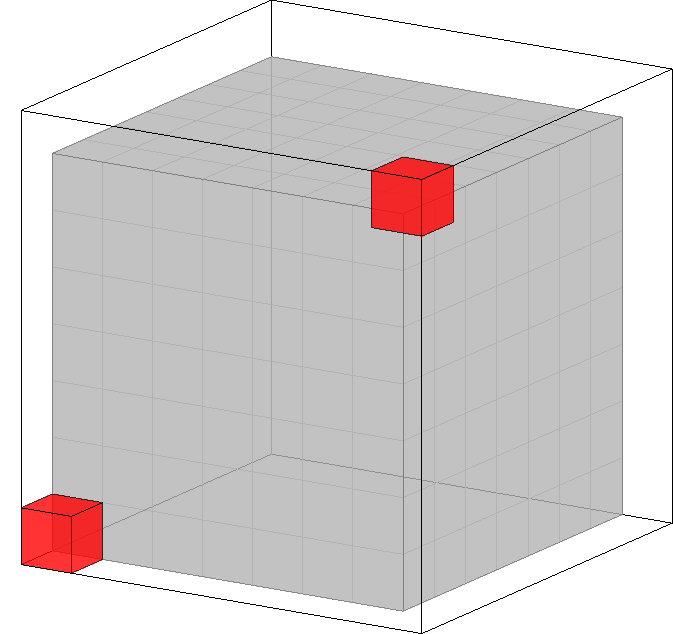
\includegraphics[width=\textwidth]{figures/1/torus.pdf}
	\caption{}
	\label{fig:torus_a}
\end{subfigure} \hfill%
\begin{subfigure}{0.21\textwidth}
	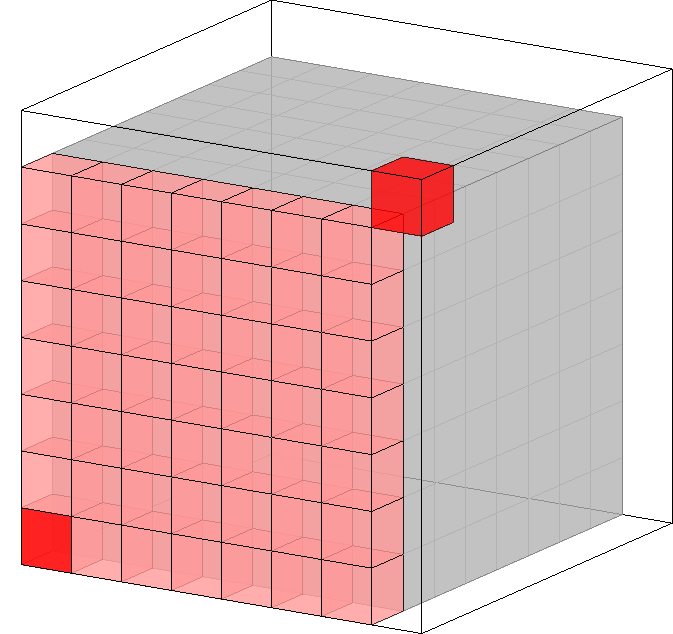
\includegraphics[width=\textwidth]{figures/1/torus_2.pdf}
	\caption{}
	\label{fig:torus_b}
\end{subfigure} \hfill
\begin{subfigure}{0.21\textwidth}
	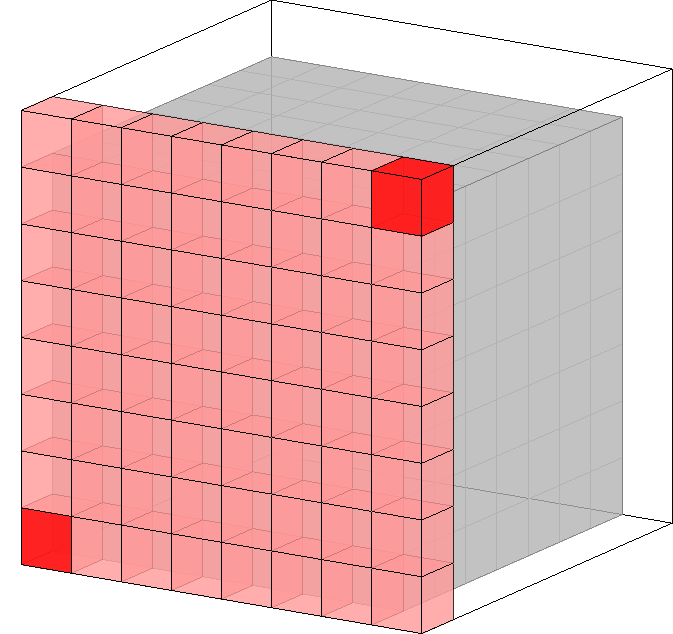
\includegraphics[width=\textwidth]{figures/1/torus_3.pdf}
	\caption{}
	\label{fig:torus_c}
\end{subfigure} \hfill
\begin{subfigure}{0.21\textwidth}
	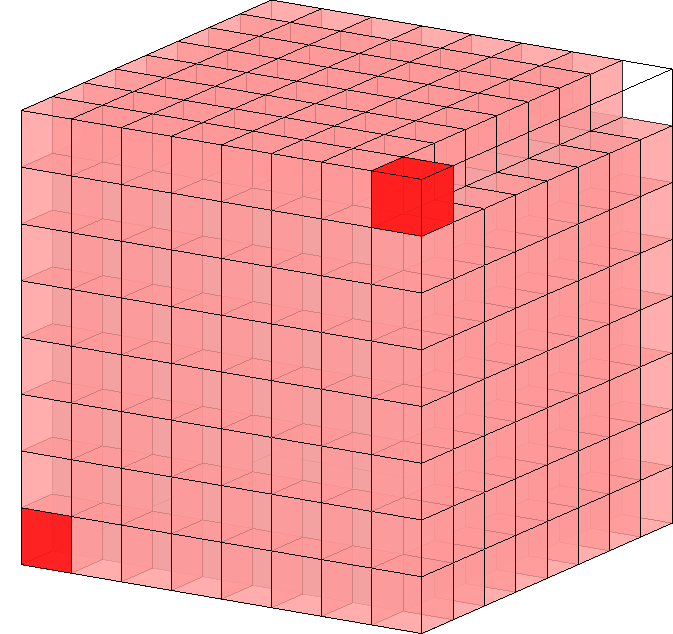
\includegraphics[width=\textwidth]{figures/1/torus_4.pdf}
	\caption{}
	\label{fig:torus_d}
\end{subfigure}
\caption{Four stages of infection on the grid $G$ (gray) inset in the larger torus, with infected vertices $u$ and $v$ (dark red).}
\label{fig:torus}
\end{figure} 

% other semi-related problems in bootstrap percolation
\subsection{Other problems}

Thus far, we have focused on the extremal problem of determining the smallest possible lethal set on $d$-dimensional grids and tori. Unsurprisingly, this is one of many existing areas of research in bootstrap percolation. In this section, we highlight a different, related problem: what is is the maximum time it takes for a lethal set to infect all vertices of a grid?

As before, we shall begin with $2$-neighbor percolation on $[n]^2$. We shall say that a lethal set $A_0 \subseteq V(G)$ percolates in time $T$ if we obtain $[A_0]$ in $T$ time-steps. For $r \in \mathbb{N}$, let
$$T(G,r) = \max\{T \in \mathbb{N} \mid \exists \text{ a set }A_0 \subseteq V(G)\text{ that }r\text{-neighbor percolates in time }T\}.$$
In 2015, Benevides and Przykucki \cite{benevides2015maximum} determined the asymptotic value of $T([n]^2,2)$. Their result is reproduced below.

\begin{thm}[Benevides, Przykucki]
The maximum percolation time on $[n]^2$ is $T([n]^2,2) = \frac{13}{18}n^2 + O(n)$. 
\end{thm}

Interestingly, this time is not achieved with minimum lethal sets (lethal sets of size $n$). In fact, the same authors showed in an earlier paper that the maximum percolation time for lethal sets $A_0$ on $[n]^2$, where $|A_0| = n$, is the nearest integer value to $\frac{5n^2-2n}{8}$ \cite{benevides2013slowly}. 

The fact that minimum lethal sets do not always percolate slowest holds for grids $[n]^2$ under 3-neighbor percolation, where $n=2^k-1$. In Chapter 5, we prove that $m([n]^2,3) = \frac{n^2+2n}{3}$ for $n=2^k-1$, and show that this is achieved for exactly one lethal configuration of vertices $A_0$. It is easy to see that $A_0$ percolates in time $(n-1)/2$ and so, if $|A_0| = \frac{n^2+2n}{3}$, then $T([n]^2,3) = \frac{n-1}{2}$ (see Figure \ref{fig:fast}). By removing the restriction on $|A_0|$, we are able to improve this to $T([n]^2,3) \geq (n-1)(n-1)/2$ (see Figure \ref{fig:slow}). It is not clear whether this lower bound is best possible; further discussion can be found in Chapter 7. 

In 2018, Hartarsky investigated maximum $r$-neighbor percolation time on $d$-dimensional hypercubes, for $r \ge 3$ \cite{hartarsky2017maximal}. In particular, they determined the following value of $T([2]^d, r)$, up to a polylogarithmic factor:

\begin{thm}[Hartarsky]
\label{thm:snakeinabox}
For all $r \ge 3$,
$$T([2]^d,r) = \frac{2^d}{d} (\log d)^{-O(1)}.$$
\end{thm}

Interestingly, the proof of Theorem \ref{thm:snakeinabox} makes use of connections between maximum induced paths in the hypercube (the Snake-in-a-Box problem) and maximum percolation time. The association between bootstrap percolation and induced paths in hypercubes was also laid out in a 2014 paper by Shende \cite{shende2015maximal}. In Chapter 7, we note that the structure of lethal sets in two-dimensional grids $[a_1] \times [a_2]$ bears resemblance to maximum induced paths in $[a_1] \times [a_2]$. 
%and, as far as we are aware, no papers have been published regarding the value of $T([n]^d,r)$ for values other than $d=r=2$. 

\begin{figure}[]
\centering
\hspace*{\fill}
\begin{subfigure}{0.3\textwidth}
	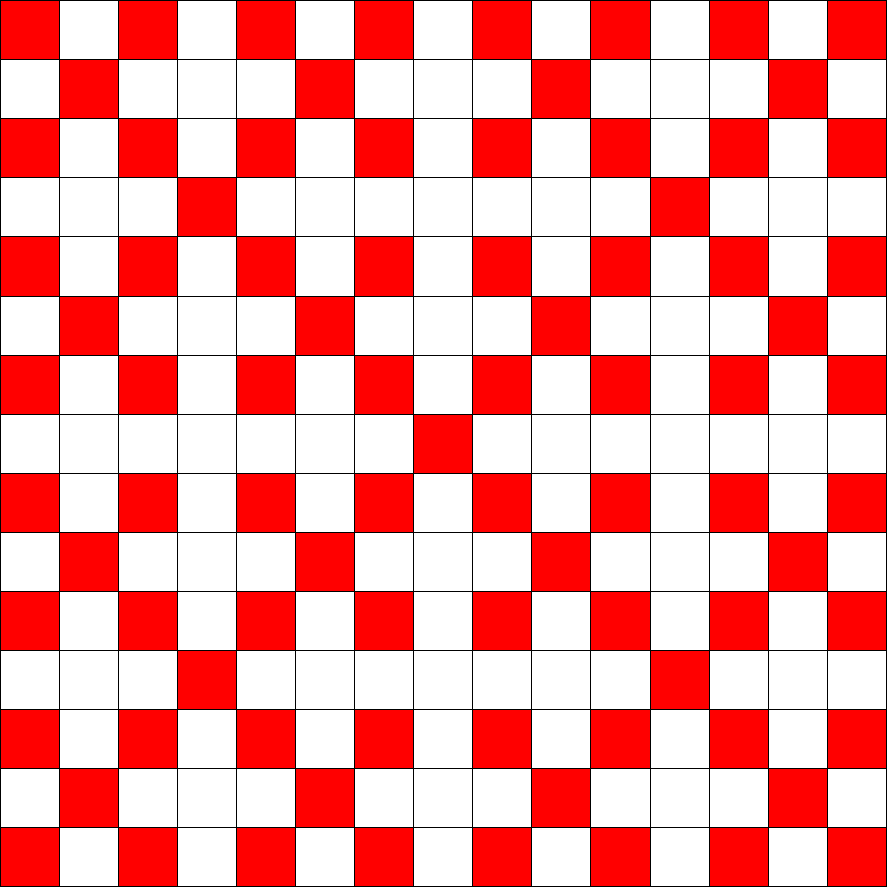
\includegraphics[width=\textwidth]{figures/1/15x15x1.pdf}
	\caption{$T([n]^2,3) = \frac{n-1}{2}$}
	\label{fig:fast}
\end{subfigure} \hfill%
\begin{subfigure}{0.3\textwidth}
	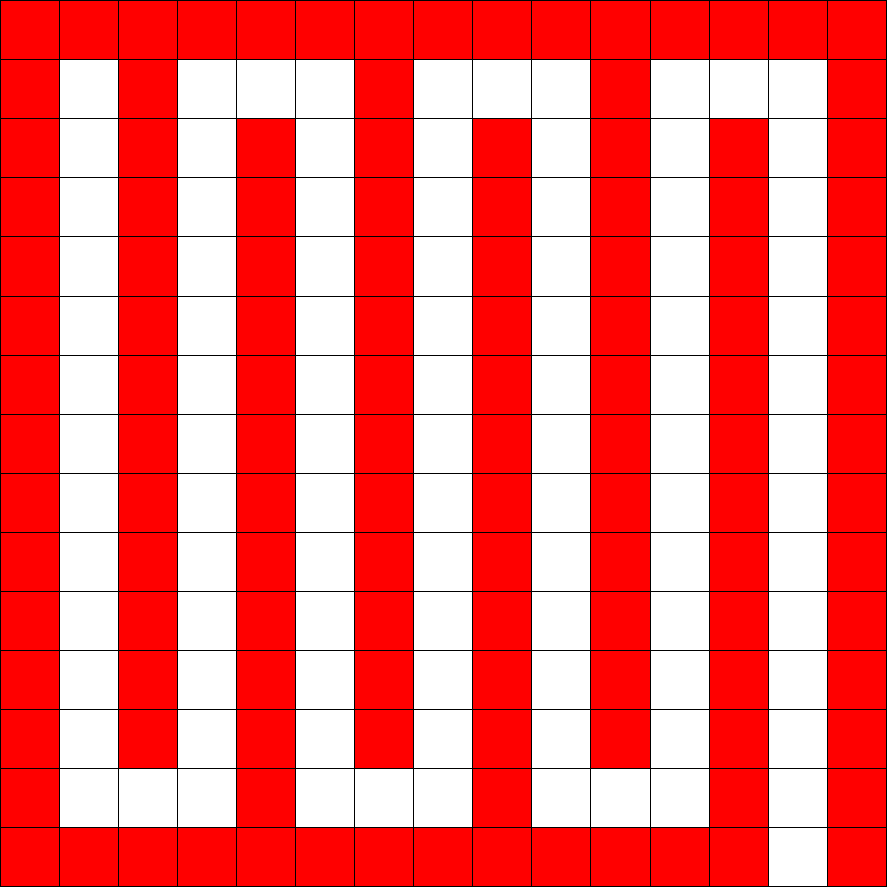
\includegraphics[width=\textwidth]{figures/1/15x15x1_slow.pdf}
	\caption{$T([n]^2,3) \geq \frac{(n-1)(n-1)}{2}$}
	\label{fig:slow}
\end{subfigure}
\hspace*{\fill}
\caption{Lethal sets on $[2^k-1]^2$ with different percolation times.}
\label{fig:percolation_time}
\end{figure} 

%In this section, we provide a cursory overview of some other related areas of study in bootstrap percolation. We highlight problems regarding the number of iterations necessary to infect all vertices on a graph.

\section{Structure of this Thesis}

As stated by Theorem \ref{thm:main_result}, the primary goal of this thesis is to prove a tight bound for 3-neighbor bootstrap percolation on three-dimensional grids of sufficiently large size. This task requires the use of two major lemmas, as well as both original and previously published ideas and constructions. In an effort to present this material in a coherent manner, the thesis is structured as follows. 

Chapters 2 and 3 are dedicated to building a conceptual and intuitive framework upon which to prove Theorem \ref{thm:main_result}. In Chapter 2, we present lemmas regarding the structure of lethal sets in both two-dimensional and $d$-dimensional grids. These lemmas will prove useful in our examination of general constructions of lethal sets (see Chapter 6). We also discuss the design and function of a visualization tool developed to assist in the examination of lethal sets. In Chapter 3, we prove a lemma that will allow us to recursively develop large families of lethal sets that match the surface area bound, and summarize all families of lethal sets that we are able to obtain. 

Chapter 4 leverages the results of Chapters 2 and 3 to prove Theorem \ref{thm:main_result}. We first show that grids $[a_1] \times [a_2] \times [a_3]$, $a_1, a_2, a_3 \geq 5$ with integral surface area bound admit tight lethal sets, and then extend this result to all grids of size 11. Chapter 5 further builds on this, highlighting some new results for 3-neighbor percolation on grids $[a_1] \times [a_2]$.

Chapter 6 and Appendix A examine the structure and lethality of percolating sets discovered in this research. In particular, Chapter 6 proves the lethality of the constructed families of sets presented in Chapter 2, and Appendix A illustrates the phases of infection on individual lethal sets.

Finally, Chapter 7 summarizes our results and provides recommendations for future research in similar and related problems. 

% proof of perimeter bound and generalization to surface area bound
% "So we have a goal, and now the question becomes whether or not it is possible to obtain this goal in all cases through constructions."

% "We shall see that generally (and especially for large grids), it is possible to find constructions that percolate at the lower bound. However, some smaller cases seem to contain unavoidable regions of immunity."
% For this reason, it will be helpful to expand on our observations about immune regions and perimeter infections."
% discussion about the notion of immune regions

% Possible discussion of existing results, where our results fit into the literature and presentation of the table??

% Lay out the structure of this paper. 
% "We show that through a clever recursive construction we are able to obtain percolating sets at the lower bound for all grids of size at least 11, and at least 5 for divisibility cases."
% "We establish a set of cases for which the lower bound cannot be met, and present a best upper bound for these cases."
% 1. Introduction
% 2. Recursion
% 3. Divisibility cases
% 4. All cases
% 5. Thickness 1
% 6. Constructions
% 7. Visualization tool??
% 8. The torus?

% vvv ONE GIANT COMMENT vvv
% COMMENT
% COMMENT
% COMMENT
% COMMENT
% COMMENT
% COMMENT
% COMMENT
% COMMENT
\begin{comment}
In the following chapter, we lay out in formal terms those lemmas necessary to understand and prove Theorem \ref{thm:main_result}. In particular, we discuss the recursive technique that permits the construction of lethal sets on grids of arbitrary large size, as well as a number of characteristics of lethal sets. We distinguish between two types of grids--those with integral \emph{SA bound}, and those without--and show that it is possible obtain tight constructions on non-integral grids from integral grids. 

In Chapter 3, we prove that there exist lethal sets at the S.A. bound for all integral grids of size at least 5. This chapter makes significant use of a number of existing constructions, described in Chapter 6, as well as the recursive strategy introduced in Chapter 2. 

Chapter 4 extends the results of Chapter 3 to all grids of size at least 11 with non-integral surface area bound. 

Chapter 5 considers the specific case of grids of the form $(a,b,1)$, and answers a question posed in Benevides et al. \cite{benevides:2021} regarding the existence of tight lethal sets on non-square grids. 

Chapter 6 is dedicated to presenting and proving the lethality of sets on a number of grids, and families of grids. 

Chapter 7 discusses some of the programmatic techniques used to evaluate, examine and explore the behavior of percolating sets. 

Chapter 8 examines the problem of bootstrap percolation on the 3- and 4-torus, and presents a class of constructions within constant size of the lower bound. 

Chapter 9 presents open questions related to the results presented in this thesis, and provides some suggestions for future research.

% COMMENT

% r=0 and r=1
\subsection{$m(G,0)$ and $m(G,1)$} 

In the case where $r \in \{0,1\}$, the specific structure of $G$ is unimportant. We have the following results:

\begin{thm}
For all undirected, simple graphs $G$, $m(G,0) = 0$.
\end{thm}

\begin{proof}
As cells need not be adjacent to infections to become infected, $A_1 = V(G)$, and so $A_0 = \emptyset$ is lethal.
\end{proof}

\begin{thm}
Let $G$ be an undirected, simple graph with $c$ components. Then $m(G, 1) = c$.
\end{thm}

\begin{proof}
Let $A_0$ be lethal. As infections spread along all edges, it is both necessary and sufficient for each connected component of $G$ to contain exactly one vertex of $A_0$. Therefore, $|A_0| = m(G,1) = c$.
\end{proof}

% r=2
\subsection{$m(G,2)$} 

We consider three classes of generalizations: the Cartesian product of paths, the Cartesian product of cycles, and the Cartesian product of both. 

\subsubsection{Grid: $P_a \square P_b$}

Recall from the discussion of Question \ref{que:simple_puzzle} that $m(n, n,2) = n$, where the tight construction for the lower bound is given by a diagonal infection expanding laterally outwards. We generalize this result to all rectangular grids.

\begin{thm}
For $a, b \geq 1$,
$$m(a,b,2) = \ceil*{\frac{a+b-2}{2}}+1.$$
\end{thm}

\begin{proof}
We obtain a lower bound on $m(a,b,2)$ by applying the perimeter argument. Note that the perimeter of the $a \times b$ grid is $2(a+b)$, and so the $m(a,b,2) \geq \ceil*{\frac{a+b}{2}} = \ceil*{\frac{a+b-2}{2}}+1$. (We take the ceiling because the size of infected sets must be integral.) For the upper bound, we generalize the construction illustrated in Figure \ref{fig:two_infections_a} to rectangular grids. Consider two cases: $a+b \equiv 0 \pmod 2$ and $a+b \equiv 1 \pmod 2$ (see Figure \ref{fig:sa_construction_2d}). Note that in both cases, the initial infectious set $A_0$ is lethal. Furthermore, note that in Figure \ref{fig:sa_construction_2d_a}, $|A_0| = \frac{a+b}{2}$, and in Figure \ref{fig:sa_construction_2d_b}, $|A_0| = \ceil*{\frac{a+b}{2}}$. In both cases, this agrees with the perimeter bound.
\end{proof}

It is worth noting that the integrality condition on the perimeter bound corresponds exactly to the non-existence of cells that are infected by more than two neighbors. In Figure \ref{fig:sa_construction_2d_a}, each cell is infected by exactly two neighboring cells; this condition ensures that $P(A_i) = P([A_0])$ for all $i$. Conversely, in Figure \ref{fig:sa_construction_2d_b}, the cell demarcated with an ``X" experiences infection on three sides. The existence of such a cell is guaranteed by the fact the perimeter bound in this case is non-integral. 

\begin{figure}[]
\centering
\begin{subfigure}{0.4\textwidth}
	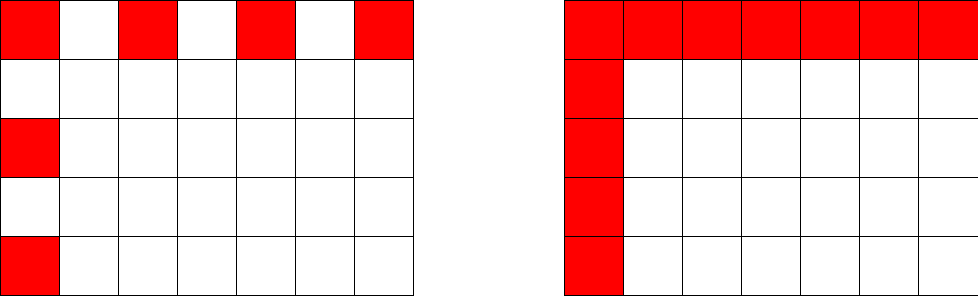
\includegraphics[width=\textwidth]{figures/1/5x7x1.pdf}
	\caption{$a+b \equiv 0 \pmod 2$}
	\label{fig:sa_construction_2d_a}
\end{subfigure} \hfill%
\begin{subfigure}{0.45\textwidth}
	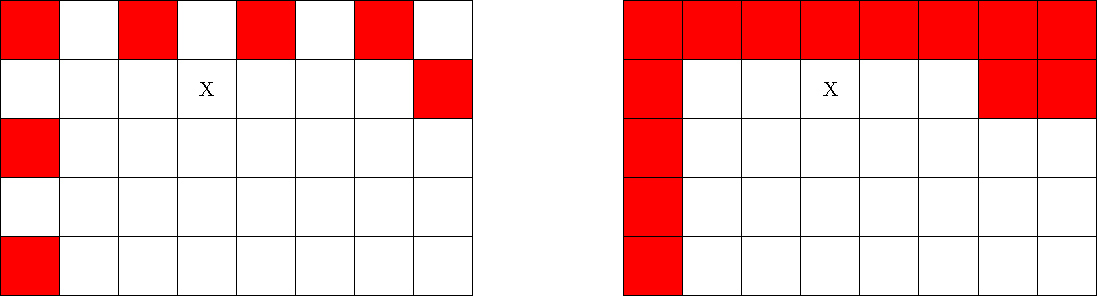
\includegraphics[width=\textwidth]{figures/1/5x8x1.pdf}
	\caption{$a+b \equiv 1 \pmod 2$}
	\label{fig:sa_construction_2d_b}
\end{subfigure}
\caption{Tight constructions for lethal sets on the $[a] \times [b]$ grid.}
\label{fig:sa_construction_2d}
\end{figure} 

\subsubsection{Grid: $P_a \square P_b \square \dots \square P_d$}

In a paper by Balogh and Bollobas \cite{balogh:2006}, the above result is generalized to all $d$-dimensional hypercubes $(a_1, \dots, a_d)$, $a_i \geq 1$. 

\begin{thm}
For $d \geq 1$ and $a_1, \dots, a_d \geq 1$, 
$$m(a_1, \dots, a_d, 2) = \ceil*{\frac{\sum_{i=1}^d (a_i-1)}{2}}+1.$$
\end{thm}

% r=3
\subsection{$m(G,3)$} 

We discuss a further generalization of the perimeter argument to higher dimensions. We show that this argument allows us to obtain nice bounds on 3-neighbor percolation in two and three-dimensional grids. We give a lower bound on the size of lethal sets in the 3-torus and 4-torus. We highlight the main theorem of this thesis.

\subsubsection{Grid: $P_n \square P_n$}

In 2021, Benevides et al. proved that 
$$m(n,n,3) = \ceil*{\frac{n^2+2n+4}{3}}$$
for even $n$, and 
$$\ceil*{\frac{n^2+2n}{3}} \leq m(n,n,3) \leq \ceil*{\frac{n^2+2n}{3}} + 1$$
for odd $n$. Additionally, they showed that these bounds are tight for odd $n$: if $n = 5 \pmod 6$, or $n = 2^k - 1$ for some $k \in \mathbb{N}$, then $m(n,n,3) = \ceil{\frac{n^2+2n}{3}}$; and if $n \in \{9,13\}$, then $m(n,n,3) = \ceil{\frac{n^2+2n}{3}} + 1$. Constructions that achieve this bound are illustrated in Chapter 5. We add to this picture with the following theorem, proven in Chapter X, and corollary:

\begin{thm}
\label{thm:2d_rectangle}
Suppose that $a, b \geq 1$ such that
$$m(a,b,3) = \frac{2ab+a+b}{3}.$$
Then there exists $k \geq 1$ such that $a=b=2^k-1$.
\end{thm}

\begin{cor}
For all $n \geq 1$,
$$ m(n,n,3) =
\begin{cases} 
      \ceil*{\frac{n^2+2n+4}{3}} & n \equiv 0 \pmod 2 \\
      \frac{n^2+2n}{3} & n = 2^k-1, \; k \in \mathbb{N} \\
      \frac{n^2+2n+1}{3} & n \equiv 5 \pmod 6 \\
      \frac{n^2+2n+3}{3} & \text{otherwise.}
   \end{cases}
$$
\end{cor}

\begin{proof}
The first three cases follow from Theorem 1 of \cite{benevides:2021} and the observation that if $n \equiv 5 \pmod 6$, then $\ceil{\frac{n^2+2n}{3}} = \frac{n^2+2n+1}{3}$. In the final case, $n$ is congruent to either 1 or 3 modulo 6. This implies that $n^2 + 2n$ is divisible by three. From Theorem 1 of \cite{benevides:2021}, we have that $m(n,n,3) \leq \frac{n^2+2n+3}{3}$. Furthermore, since $n$ is not of the form $2^k-1$, it follows from Theorem \ref{thm:2d_rectangle} that $m(n,n,3) > \frac{n^2+2n}{3}$. Therefore, $m(n,n,3) = \frac{n^2+2n+3}{3}$.
\end{proof}

This result resolves the question of the minimum lethal set for two dimensional square grids. For the more general case of rectangular grids, the problem remains unsolved. However, we are able to achieve an upper bound of $m(a,b,3) \leq \ceil{\frac{ab+a+b+6}{3}}$ for all $a,b > 1$. Further discussion of these results can be found in Chapter X.

\subsubsection{Grid: $P_a \square P_b \square P_c$}

%Observe that the surface area bound presented above applies directly to 3-dimensional grids. State the main theorem of this thesis. 
Surprisingly, it is possible to extend the perimeter argument to higher dimensions \cite{przykucki:2019}. This provides a lower bound on $m(a_1,a_2,a_3,3)$ of $\ceil{\frac{a_1a_2+a_2a_3+a_1a_3}{3}}$. We refer to this quantity as the \emph{surface area bound}. In Chapters 2 and 3, we use a recursive strategy to prove that the surface area bound is met for all sufficiently large grids. 

\begin{thm}
\label{thm:main_result}
For all $a_1, a_2, a_3 \geq 11$, 
$$m(a_1,a_2,a_3,3) = \ceil*{\frac{a_1a_2+a_2a_3+a_1a_3}{3}}.$$
\end{thm}

\subsubsection{Grid: $P_a \square P_b \square \dots \square P_d$}

Do we have a bound here?

\subsubsection{Torus: $C_a \square C_b$}

A lower bound for the Cartesian product of two cycles is given in Benevides \cite{benevides:2021}. Their proof is included here for completeness.

\begin{thm}
\label{thm:torus_lb}
For $a, b \geq 1$,
$$m(C_a \square C_b,3) \geq \ceil*{\frac{ab +1}{3}}.$$
\end{thm}

\begin{proof}
Let $G = C_a \square C_b$, and let $I$ be a lethal set on $G$. Let $H = V(G) \setminus I$, and note that $|H| = ab - |I|$. Let $m_{H}$ be the number of edges in the subgraph of $G$ induced by $H$, and $m_{IH}$ be the number of edges between vertices in $I$ and vertices in $H$. Note that $m_{IH}$ is similar to the notion of perimeter on a grid.

Observe that $G[H]$ must be cycle-free: cycles in $G[H]$ constitute immune regions, and contradict the lethality of $I$. Therefore, $G[H]$ is a forest, and so $m_H = |H| - c$, where $c$ is the number of components in $G[H]$. Additionally, note that $m_{IH} \leq 4|I|$, since $G$ is $4$-regular. Finally, observe that the total degree of $G[H]$ is $2m_H = 4|H| - m_{IH}$.

Chaining together these inequalities, we obtain:
\begin{align*}
4|I| \geq m_{IH} &= 4|H| - 2m_H \\
&= 4|H| - 2(|H| -c) = 2|H| + 2c \\
&= 2(ab-|I|) + 2c
\end{align*}
Combining like terms and simplifying, we have
$$|I| \geq \frac{ab +c}{3} \geq \frac{ab +1}{3}.$$
\end{proof}

Observe that the conditions $c \geq 1$ and $m_{IH} \leq 4|I|$ prevent us from obtaining strict equality. Specifically, if $I$ is lethal, $G[H]$ has one component, and no vertices in $I$ are adjacent, then $|I|$ is minimized. 

\subsubsection{Torus: $C_a \square C_b \square C_c$}

Present the lower bound and note that we are able to obtain constructions within constant distance of this bound for arbitrarily large grids.

%In the context of question \ref{que:simple_puzzle}, $G = P_{10} \Osq P_{10}$, and our diagonal construction shows us that $m(2,G) \leq 10$. In general, we have observed that for $G = P_n \Osq P_n$, $m(2, G) \leq n$. Now, let us prove that the bound is, in fact, tight. 

\begin{prop}
\label{prop:tight_perimeter}
For all $n \geq 1$, 
$$m([n]^2, 2) = n.$$
\end{prop}

\begin{proof}
The upper bound follows from our diagonal construction in figure \ref{fig:two_infections} (\subref{fig:two_infections_b}). The lower bound is given by the famous ``perimeter argument". Consider the $n\times n$ grid $G$, given by $G = P_n \Osq P_n$. Let $A_0 \subseteq V(G)$ be a set of initially infected cells. We claim that the total perimeter of all infected regions in $G$ is monotonically decreasing as a function of the time-step $t$. Consider an arbitrary healthy cell $c$. In order for $c$ to become infected, at least two of its edges must abut infected cells. However, this implies that (upon infection of $c$) these edges are absorbed within the newly expanded infected region, thereby reducing the perimeter of infection by two. As $c$ contains at most two un-absorbed edges, the perimeter of infection cannot increase. 

Since a lethal set will infect the entire grid, and therefore have a final perimeter of infection of $4n$, it follows that the perimeter of infection of $A_0$ must be at least $4n$, and so $m([n]^2, 2) \geq n.$
\end{proof}

This proof appears in \cite{przykucki:2019}, although it has been an established result in bootstrap percolation ``folklore" for considerably longer. We should like to make a few additional observations. 

First, note that we have used the following three expressions to describe the same graph $G$:

\begin{center}
\begin{enumerate*}[label=\roman*),itemjoin={\qquad}]
\item $n \times n$
\item $P_n \Osq P_n$
\item $[n]^2.$
\end{enumerate*}
\end{center}
\vspace{0.2in}

\noindent The notation in (i) is useful when discussing the shape of low dimensional, asymmetric grids. We use the notation in (ii) to remind readers that the fundamental structure in bootstrap percolation problems is a graph, and to suggest possible extensions of the problem discussed in this thesis to other similar objects. The notation in (iii) is the standard way to describe the vertex set of a grid graph, and can readily be generalized to any dimension $d$ by writing $[n]^d$. In a slight abuse of notation, we use $[n]^d$ to represent the entire graph $G$, and draw edges between vertices that differ by exactly one in exactly one coordinate. 

Second, the fact that we have used the notation $[n]^2$ in Proposition \ref{prop:tight_perimeter} suggests that we can generalize to higher dimensional grids $[n]^d$. Indeed, simply observe that for a given hypercube cell to become infected, it must donate at least $d$ of its $2d$ hyperplane faces to the infected region, thereby at most maintaining the current $(d-1)$-perimeter of infection. The following theorem summarizes this result.  

\begin{thm}
\label{thm:square_sa_bound}
For all $n,d \geq 1$, 
$$m([n]^d, d) \geq n^{d-1}.$$
\end{thm}

More generally, denote by $(a_1, \dots, a_n)$ the grid graph with vertex set $V = \{(i_1,\dots,i_n) \mid i_1 \in [a_1], \dots, i_n \in [a_n]\}$, and edge set $E = \{uv \mid u,v \text{ differ by one in exactly one coordinate}\}$. The following theorem provides a general lower bound on the size of lethal sets for all such graphs. 

\begin{thm}
\label{thm:general_sa_bound}
Let $G = (a_1, \dots, a_d)$, for $a_1, \dots, a_d, d \geq 1$. Then:
$$m(G, d) \geq \text{ sum of products of all subsets of size d-1, divided by d}.$$
\end{thm}

\begin{proof}
The proof follows the same high-dimensional surface area argument outlined above. 
\end{proof}

We highlight the three-dimensional instance of Theorem \ref{thm:general_sa_bound} in Corollary \ref{cor:sa_bound}, as it will prove particularly useful in the following chapters. We refer to this bound as the \emph{surface area} or \emph{S.A. bound}.

\begin{cor}
\label{cor:sa_bound}
Let $G = (a, b, c)$, for $a, b, c \geq 1$. Then:
$$m(G, 3) \geq \ceil*{\frac{ab + bc + ca}{3}}.$$
\end{cor}

\begin{proof}
Follows directly from Theorem \ref{thm:general_sa_bound}.
\end{proof}

While it has been shown that tight constructions exist for grids of the form $[n]^d$, where $r=d$, the problem of determining the existence of similar constructions for rectangular grids remains unsolved. In this thesis, we focus our attention on the particular case of $d=3$ and show that $m(a,b,c, 3) = \ceil*{\frac{ab + bc + ca}{3}}$ for all $a,b,c \geq 11$. 

% Separation of two commented out sections
% COMMENT
% COMMENT
% COMMENT
% COMMENT
% COMMENT

The problem of bootstrap percolation was first introduced in the 1970s by Chalupa et al. \cite{chalupa:1979} as a simplified model for the behavior of ferromagnetic fields. In their original paper, the authors describe bootstrap percolation as the stabilization of a probabilistically occupied lattice, where each occupied site must be adjacent to at least $m$ occupied neighbors. A re-rendering of the examples given in the original 1979 paper is presented in figures 1 and 2. 

In this original problem, the authors are interested in the structural patterns of these stable arrangements. Put differently, given a set of randomly distributed occupants on a $d$-dimensional lattice, what configuration can we expect these occupied sites to fall into, subject to the constraint that each occupied site is adjacent to at least $m$ other occupants? In this construction, a probabilistically populated lattice is iteratively de-populated until it reaches a stable state. 

Alternatively, we might consider the behavior of a population as it grows, instead of shrinks. In this model, it is useful to consider the population as harboring an infection that steadily spreads from site to site, subject to population density. We shall consider these infections to take place on a graph, with vertices representing members of our population (sites), and edges indicating adjacency. In formal terms: let $G$ be a graph and $A_0 \subseteq V(G)$ be a set of initially infected vertices. Iteratively, at every time step, infect those vertices of $G$ with at least $r$ infected neighbors. For all $t > 0$, let $A_t$ be the set of infected vertices at time step $t$. We then have
$$A_t = A_{t-1} \cup \{v \in V(G) : |N_G(v) \cap A_{t-1} \geq r\},$$
where $N_G(v)$ is the set of vertices adjacent to $v$ in $G$. We define the \emph{closure} of $A_0$ under $r$-neighbor bootstrap percolation to be $[A_0] = \bigcup_{t=0}^{\infty} A_t$. This is analogous to the stable states introduced in \cite{chalupa:1979}. We say that $A_0$ \emph{percolates} or is \emph{lethal} if $[A_0] = V(G)$. We note that under these rules, it is not possible for vertices to become uninfected. 

Perhaps the most natural extremal question regarding $r$-neighbor bootstrap percolation is that of determining the size of the smallest percolating set $A_0 \subseteq V(G)$, for a given graph $G$. We represent this quantity by $m(G,r)$. There has been a great deal of work done on establishing the value of $m(G,r)$ for various classes of graphs and values of $r$ (see \{citations, citations, etc., etc.\}). These results are incompletely summarized in table \ref{tab:known_bounds}, and a selection of particularly noteworthy proofs are presented in detail in the following section.

\begin{table}[]
\centering
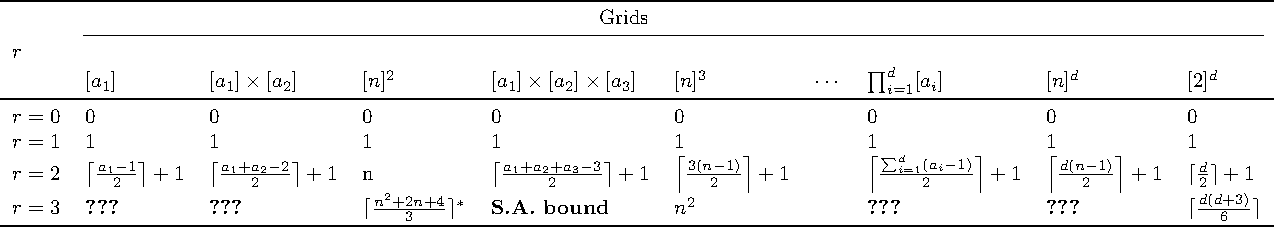
\includegraphics[width=\textwidth,origin=c]{tables/1/known_bounds.pdf}
\caption{A summary of known bootstrap percolation results for grids and the torus, $r \in \{0,1,2,3,d\}$.}
\label{tab:known_bounds}
\end{table} 

We end this introduction with the presentation of a delightful question about the cardinality of $2$-neighbor percolating sets on the two-dimensional lattice. The interested reader in encouraged to find a solution on their own; however, a proof of the result is presented at the beginning of the following section.
\begin{question}
Let $(n,n)$ represent the $n \times n$ lattice, given by $G = P_n \times P_n$. What is $m(n,n,2)$?
\end{question}

\section{Minimum percolating sets and bounds}

\subsection{Foundations}

Let us build some intuition for the behavior of percolating sets on the two-dimensional lattice. Figure \ref{fig:5x5x1} illustrates the percolation time-steps for an arbitrary initial infection on the graph $G=P_5 \times P_5$, where $r=2$. (In general, we shall refer to the $d$-dimensional lattice with sides $a_1, \dots, a_d$ as the $d$-tuple $(a_1, \dots, a_d)$. The standard notation is $\prod_{i=1}^d a_i$.) 

\begin{figure}[]
\centering
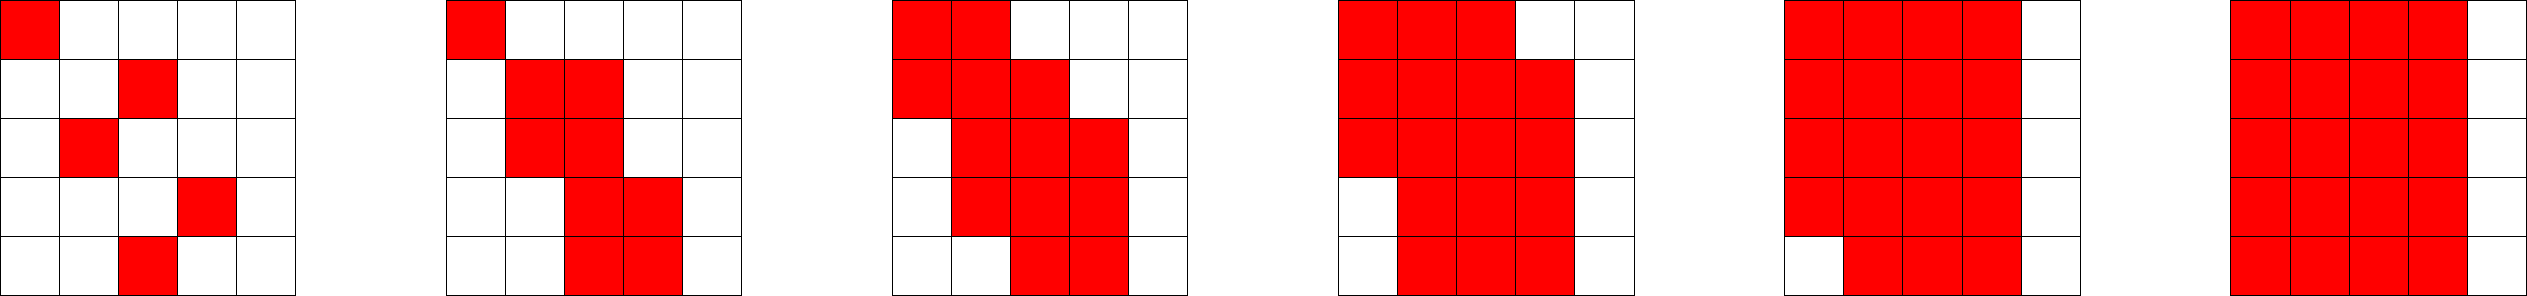
\includegraphics[width=\textwidth]{figures/1/5x5x1.pdf}
\caption{Percolation time-steps for an arbitrary initial infection on the $5 \times 5$ lattice, $r=2$.}
\label{fig:5x5x1}
\end{figure} 

Note that this configuration fails to infect the entire grid; that is, the initial infection is not lethal. Heuristically, this appears to be a consequence of the fact that infected cells are unable to access the healthy cells in the rightmost column. We might, therefore, hypothesize that an initial infection must somehow ``span" the entire lattice. A potential ``spanning" construction is illustrated in figure \ref{fig:5x5x1_improved}. Observe that at each time-step, the infection spreads out laterally from the initial diagonal. It is a simple exercise to verify that this construction is lethal on all $(n,n)$ grids for $r=2$. We also note that a similar construction is lethal on all $(n,m)$ grids for $r=2$ (figure \ref{fig:8x4x1}).

\begin{figure}[]
\centering
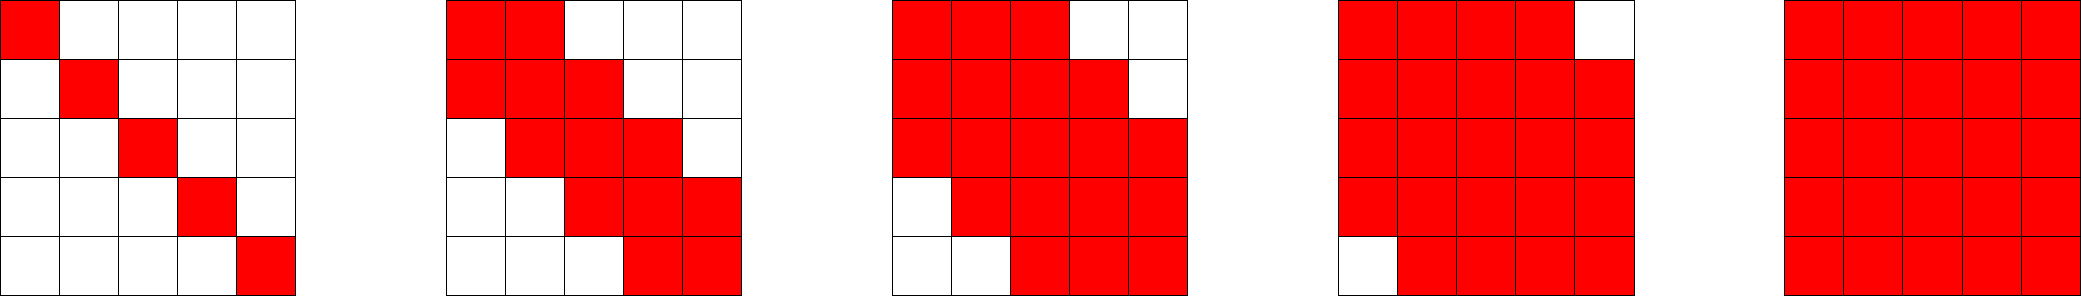
\includegraphics[width=\textwidth]{figures/1/5x5x1_improved.pdf}
\caption{Percolation time-steps for a ``spanning" initial infection on the $5 \times 5$ lattice, $r=2$.}
\label{fig:5x5x1_improved}
\end{figure} 

\begin{figure}[]
\centering
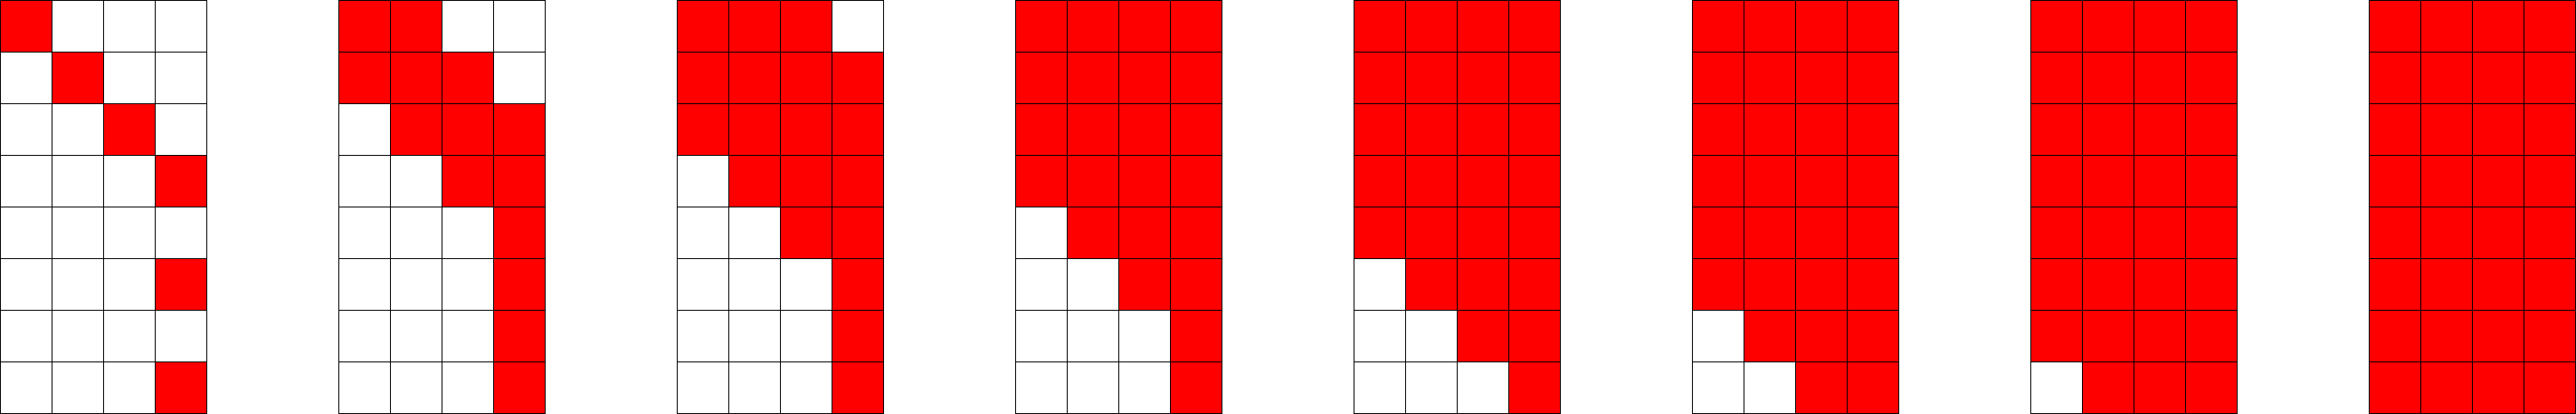
\includegraphics[width=\textwidth]{figures/1/8x4x1.pdf}
\caption{A lethal infection on the $8 \times 4$ lattice, $r=2$.}
\label{fig:8x4x1}
\end{figure} 

The $(n,n)$ construction can be generalized to any dimension. Specifically, we have:

\begin{prop}
\label{prop:nxn_lower_bound}
For all $n,d \geq 1$, 
$$m([n]^d, d) \leq n^{d-1}.$$
\end{prop}
This result has been known since at least Pete \cite{pete:1997}, although the particular constructions are difficult to render in general. The following proof (appearing in \cite{przykucki:2019}, but known in bootstrap percolation ``folklore" for much longer) elegantly shows that this bound is tight.

\begin{thm}
\label{thm:tight_perimeter}
For all $n,d \geq 1$, 
$$m([n]^d, d) = n^{d-1}.$$
\end{thm}

\begin{proof}
The upper bound follows from proposition \ref{prop:nxn_lower_bound}. The lower bound is given by a generalization of the famous ``perimeter argument". Suppose $d=2$ and consider an embedding of $G=[n]^d$ in the $n\times n$ grid. Let $A_0 \subseteq V(G)$ be a set of initially infected cells. We claim that the total perimeter of all infected regions in $G$ is monotonically decreasing as a function of the time-step $t$. Consider an arbitrary healthy cell $c$. In order for $c$ to become infected, at least two of its edges must abut infected cells. However, this implies that (upon infection of $c$) these edges are absorbed within the newly expanded infected region, thereby reducing the perimeter of infection by two. As $c$ contains at most two un-absorbed edges, the perimeter of infection cannot increase. 

Since a lethal set will infect the entire grid, and therefore have a final perimeter of infection of $4n$, it follows that the perimeter of infection of $A_0$ must be at least $4n$, and so $m([n]^2, 2) \geq n.$

The same argument generalizes nicely to higher dimensions. Simply observe that for a given hypercube cell to become infected, it must donate at least $d$ of its $2d$ hyperplane faces to the infected region, thereby at most maintaining the current $(d-1)$-perimeter of infection.
\end{proof}

We note that the perimeter argument extends directly to rectangular grids; however, the problem of obtaining tight constructions, should they exist, is largely unsolved and will be the main focus of this thesis. The following proposition, which we refer to informally as the \emph{surface area bound} or \emph{S.A. bound}, provides a lower bound on the size of lethal sets for $d$-dimensional rectangular grids where $r=d$.

\begin{prop}
\label{prop:SA_bound}
For $d \geq 1$ and $a_1, \dots, a_d \geq 1$,
$$m(a_1, \dots, a_d, d) \leq \frac{\sum_{i=1}^d \prod_{j \neq i} a_j}{d}.$$
\end{prop}

\begin{proof}
Observe that the expression
$$\frac{\sum_{i=1}^d \prod_{j \neq i} a_j}{d}$$
is precisely the high-dimensional perimeter of the grid graph $(a_1, \dots, a_d)$. The bound follows from the perimeter argument in theorem \ref{thm:tight_perimeter}. 
\end{proof}

In \{some chapter of this thesis\}, we will prove that this bound is tight in the case where $d=3$ and $d_1,d_2,d_3 \geq 8$. We fully expect that this bound can be incrementally diminished; however, we feel that such small improvements do not at this time justify the effort required to obtain additional constructions. 

In the remainder of this section, we shall present a number of additional bootstrap percolation results for different classes of grid graphs.

\subsection{Additional results}

Recall from the previous section that $m(n,n,2) = n$, where the tight construction for the lower bound is given by a diagonal infection expanding laterally outwards. In a paper by Balogh and Bollobas \cite{balogh:2006}, this result is generalized to all $d$-dimensional hypercubes $(a_1, \dots, a_d)$, $a_i \geq 1$. 

\begin{thm}
For $d \geq 1$ and $a_1, \dots, a_d \geq 1$, 
$$m(a_1, \dots, a_d, 2) = \ceil*{\frac{\sum_{i=1}^d (a_i-1)}{2}}+1.$$
\end{thm}

\begin{proof}
\end{proof}

As suggested by table \ref{tab:known_bounds}, general results become quite sparse for $r \notin \{2,d\}$. A nice result from Morrison and Noel resolves the question of $r=3$ for hypercubes $P_2^d$ of dimension $d \geq 3$. 

\begin{thm}
For $d \geq 3$ and $a_1 = \dots = a_d = 2$, 
$$m(a_1, \dots, a_d, 3) = \ceil*{\frac{d(d+3)}{6}}.$$
\end{thm}

\begin{proof}
\end{proof}

However, the issue of determining $m(a_1, \dots, a_d, r)$ is largely unresolved. Furthermore, good lower bounds for $r \neq d$ are conspicuously absent. 
\end{comment}
% ^^^ ONE GIANT COMMENT ^^^
% COMMENT
% COMMENT
% COMMENT
% COMMENT
% COMMENT

